\subsection{Caso de uso 6.1: Activar y desactivar usuarios} \label{cu}
\subsubsection{Resumen}
\subsubsection{Descripción}
En este caso de uso le permite al activar y/o desactivar un usuario
\begingroup
\setlength{\LTleft}{-10cm plus -1fill}
\setlength{\LTright}{\LTleft}
\begin{center}
  \captionof{table}{Caso de uso 6.1: Activar y desactivar usuarios} \label{tab:cu_tab}
  \begin{longtable}{| p{3.5cm} | p{11.5cm} |}
        \hline
        \textbf{Versión} & 0.1 \\
        \hline 
        \textbf{Autor} & \\
        \hline
          \textbf{Estatus} & Edicion\\
        \hline  
          \textbf{Fecha de último estatus} &  31 de marzo de 2017\\
        \hline
      \multicolumn{2}{c |}{\large{Atributos:}} \\
        \hline
          \textbf{Actor}  &  Administrador\\
        \hline  
          \textbf{Propósito} &  Permite al administrador decidir que cuentas activar y cuales desactivar\\
        \hline
          \textbf{Disparador} & \\
        \hline  
          \textbf{Entradas} & 
              \begin{itemize}
                \item Id usuario: Se escribe con el teclado.
              \end{itemize} \\
        \hline  
          \textbf{Salidas} & 
              \begin{itemize}
                \item Interna: Se mostrará el mensaje que indica que el usuario ha sido activado o desactivado
              \end{itemize} \\
        \hline  
          \textbf{Precondiciones} &
              \begin{itemize}
                \item \textbf{Interna:} El administrador debe ingresar al sistema
              \end{itemize} \\
        \hline  
          \textbf{Postcondiciones} &
              \begin{itemize}
                \item \textbf{Interna:} Un mensaje de confirmación de la operación
              \end{itemize} \\
        \hline
          \textbf{Reglas de negocio} &
              \begin{itemize}
                 \item {\hyperref[rnr_04]{RNR 04: Campos obligatorios}}
              \end{itemize} \\
        \hline
          \textbf{Mensajes} &
              \begin{itemize}
                 \item {\hyperref[msja_01]{MSJA 01: Campos en blanco}}
              \end{itemize} \\
        \hline
          \textbf{Tipo} & Secundario\\
        \hline      
  \end{longtable}
\end{center}
\endgroup

\subsubsection{Trayectorias del caso de uso}
\textbf{Trayectoria principal}
\begin{enumerate}
  \item {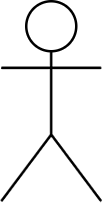
\includegraphics[scale=.1]{Capitulo3/img/actor.png} Ingresa el administrador al portal web mediante una dirección eletrónica.}
  \item {
\includegraphics[scale=.05]{Capitulo3/img/proceso.png} Se muestra la vista IU Index para el administrador.}
  \item {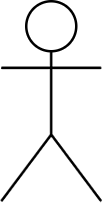
\includegraphics[scale=.1]{Capitulo3/img/actor.png} Presiona el botón de Iniciar sesión.}
  \item {
\includegraphics[scale=.05]{Capitulo3/img/proceso.png} Se muestra la vista IU Index.}
  \item {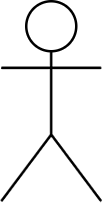
\includegraphics[scale=.1]{Capitulo3/img/actor.png} Selecciona el administrador el botón \textit{Activar/Desactivar cuentas}}
  \item {
\includegraphics[scale=.05]{Capitulo3/img/proceso.png} Se muestra la vista IU}
  \item {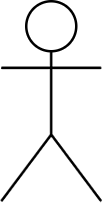
\includegraphics[scale=.1]{Capitulo3/img/actor.png} El actor ingresa el Id de la cuenta a desactivar o activar 
  \item {
\includegraphics[scale=.05]{Capitulo3/img/proceso.png} Se muestra un mensaje de confirmación del proceso }
  \textit{Fin de caso de uso} \\  
\end{enumerate}

\textbf{Trayectoria alternativa} \phantomsection\label{cu_ta_} \\
\textbf{Condición:} \\
 \begin{enumerate}[label=\arabic*]
    \item {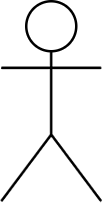
\includegraphics[scale=.1]{Capitulo3/img/actor.png} }
    \item {
\includegraphics[scale=.05]{Capitulo3/img/proceso.png}}
    \item {Continua en el paso 4 de la trayectoria principal.} \\
    \textit{Fin de trayectoria} \\
\end{enumerate}

\subsubsection{Puntos de extensión}
\noindent \textbf{Causa de la extensión: El actor, de tipo administrador selecciona \textit{Activar o Desactivar usuarios} } \\
\textbf{Región de la trayectoria:} \hyperref[cu_ta_]{Trayectoria alternativa } \\
\textbf{Extiende a:} \hyperref[cu6]{CU 6 Consultar usuarios}
